\chapter{Introduction}\label{chapter:introduction}

\section{Motivation}
In recent years,the Internet of Things(IoT) has gathered significant traction which has led to the exponential increase in the number of devices connected to the internet. According to a report released by Cisco, it is estimated that a total of 50 million devices will be
connected to the internet by the year 2020. Data is generated in an enormous amount in real-time by sensors and actuators contained in these devices. With the vast amounts of connected heterogeneous devices,
security and privacy risks are exponentially increased. Rapid7 \cite{rapid7}, an  internet security and analytics organization, released a report highlighting vulnerabilities that exists on select IoT devices. In their report, they outline  vulnerabilities in
baby monitors which allowed intruders unauthorized access to devices
whereby a malicious intruder can view live feeds from a remote location. Having a provenance aware device will be of immense benefit to the security of the device since it ensures trust between interconnected devices. With Provenance information, we can generate an activity trail which can be further analyzed to determine the who, where, and how, in the event of a malicious activity \cite{cheney_provenance_2009}. 
\par In an IoT system, most of the interconnected heterogeneous devices (things) are embedded systems which
require lightweight and efficient solutions as compared to general purpose
systems.This requirement is attributed to the constrained memory and computing power of such
devices. A major issue arise in ensuring that data is properly secured and
disseminated across an IoT architecture. The vast amount of data generated from IoT
devices requires stronger levels of trust which can be achieved through data
provenance. Provenance is used to determine causality and effect of 
operations performed on data objects \cite{glavic_case_2011}. Data provenance ensures
authenticity, integrity and transparency between information disseminated across an
IoT system.This level of transparency can be translated to various levels across the IoT architectural stack.To achieve transparency in an IoT framework, it is imperative that data provenance and IoT systems be combined to create a provenance aware system that provides detailed records of all data
transactions performed on devices connected in an IoT network.






\section{Provenance-Aware IoT Device Use Case}

\begin{figure}[h]
\begin{center}
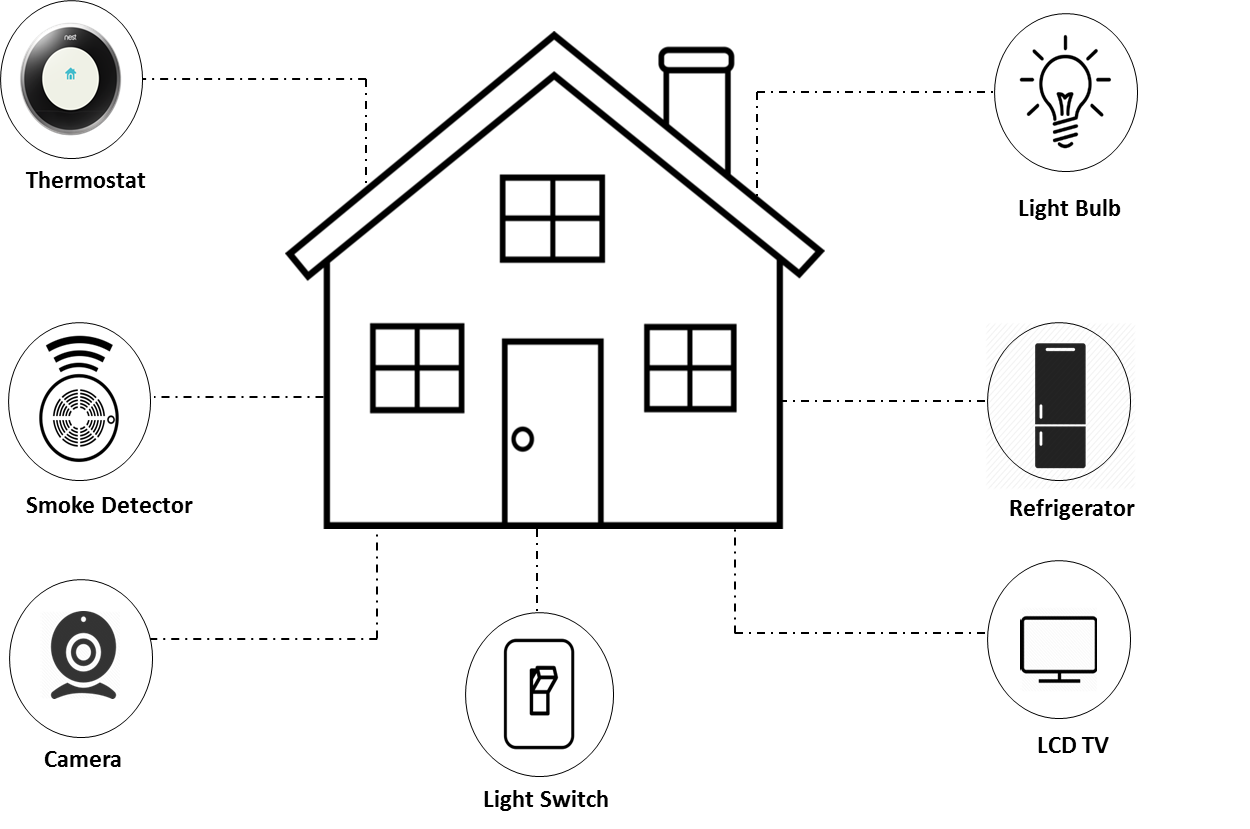
\includegraphics[height=3in]{smart_h.png}
\end{center}
\caption{Smart home use case Diagram}
\end{figure}


Consider a smart home which contains interconnected devices such as a thermostat connected a wireless network which automatically detects and regulates the temperature of a room based on prior information of a user's temperature settings, a smart lock system which can be controlled remotely and informs a user via short messaging when a breach has occurred, a home security camera motoring system, A smart fridge which sends a reminder when food produce are low. A malicious intruder successfully attempts  to gain access to the smart lock system and security camera remotely. Provenance can be used to track the series  of events to determine where and how a malicious attack originated.It can also be used as a safeguard to alert of a possible remote or insider compromise thereby protecting future or current malicious attacks. 





\section{Research Questions}
Data provenance and IoT are two important components that need to be unified. However, the unification of data provenance and IoT raises some important research issues. Some of which are as a result of preexisting provenance and IoT issues. Some of the issues raised as a result of the unification of data provenance with IoT are outlined below:

\begin{itemize}

\item Memory constraints on IoT Devices: The vast amounts of data generated leads high storage space utilization . Proper memory management/data pruning techniques should be employed for efficient storage of provenance data on memory constrained devices. 

\item A fundamental question exists in effective modeling of provenance data. How do we model provenance data collected for IoT devices? Are there models used to represent causality between sensor and actuator readings in the IoT architecture.

\item How do we effectively collect provenance data in resource constrained device and relate this information accross various layer of the IoT architecture

\end{itemize}

\section{Research Contribution}

In this dissertation, we propose the following key contributions:

\begin{itemize}
  \item A provenance collection framework which denotes causality and dependencies between entities contained in an IoT system.This system creates the groundwork for capturing and storing provenance data  on IoT devices.
  \item An efficient algorithm for storing provenance data on IoT devices. We evaluate our contributions for an efficient provenance storage by using an intrusion detection system on IoT devices.
\end{itemize}

\section{Organization of Dissertation proposal}

The remaining portion of the dissertation proposal is organized as follows.  Chapter 2 talks about background information on data provenance and the internet of things. It also discusses the models for representing provenance data and an overview of relevant compression techniques. Chapter 3 discusses the literature review on the state of the art on provenance collection in file systems, scientific workflows and database systems. Chapter 4 talks about our proposed provenance collection system. Chapter 5 describes our framework for efficient storage of provenance data. Chapter 6 concludes the proposal and proposed future work in the research.

